%% LyX 2.3.7 created this file.  For more info, see http://www.lyx.org/.
%% Do not edit unless you really know what you are doing.
\documentclass[english]{article}
\usepackage[T1]{fontenc}
\usepackage[latin9]{inputenc}
\usepackage{amsmath}
\usepackage{amssymb}
\usepackage{stackrel}
\usepackage{graphicx}

\makeatletter
%%%%%%%%%%%%%%%%%%%%%%%%%%%%%% User specified LaTeX commands.
%=====================================================================
% Identification
%=====================================================================
\NeedsTeXFormat{LaTeX2e}

\RequirePackage{fancyhdr}
\RequirePackage[top=1in,bottom=1in,left=1in,right=1in]{geometry}
\RequirePackage{graphicx}
\RequirePackage{empheq}
\RequirePackage{ifthen}


%\RequirePackage{jhwgraphics} Another personal style file I use.


%=====================================================================
% Commands
%=====================================================================

  \setlength{\headheight}{15pt}
  \lhead{\@author}\chead{\@title}\rhead{Miscellaneous}
%{\today}
  \lfoot{}\cfoot{\thepage}\rfoot{}
  \pagestyle{fancy}

  }
                                          %PDFLaTeX
  \RequirePackage[pdftex,bookmarks=true]{hyperref}
  \hypersetup{ %
    pdfauthor   = {\@author},
    pdftitle    = {\@title},
    pdfcreator  = {LaTeX with hyperref package},
    pdfproducer = {dvips + ps2pdf}
  }
\pdfadjustspacing=1

\makeatother

\usepackage{babel}
\begin{document}

\section*{Summation identities}
\begin{itemize}
\item $e^{x}=\mathop{\stackrel[k=0]{\infty}{\sum}\frac{x^{k}}{k!}}$
\item $\frac{1}{1+x}=\mathop{\stackrel[k=0]{\infty}{\sum}(-1)^{k}x^{k}}$
for $|x|<1$
\item $\stackrel[x=1]{n}{\sum}x=\frac{n(n+1)}{2}$
\item $\stackrel[x=1]{n}{\sum}x^{2}=\frac{n(n+1)(2n+1)}{6}$
\item $\stackrel[k=0]{n}{\sum}{n \choose k}=2^{n}$
\item $\stackrel[k=0]{n}{\sum}{n \choose k}a^{k}b^{n-k}=(a+b)^{n}$ (binomial
theorem)
\item $\stackrel[k=0]{n}{\sum}(-1)^{k}{n \choose k}=0$
\item $\stackrel[k=1]{n}{\sum}k{n \choose k}=n2^{n-1}$
\item $\stackrel[k=1]{n-1}{\sum}x^{k}=\frac{x^{n}-1}{x-1}$ applicable when
$x\neq1$
\item $\stackrel[k=0]{\infty}{\sum}x^{k}=\frac{1}{1-x}$ for $x\in(-1,1)$
\item $\stackrel[k=1]{n}{\sum}\frac{1}{2^{k}}\rightarrow1$
\item $\int_{x}^{\infty}\frac{1}{\Gamma(\alpha)}z^{\alpha-1}e^{-z}dz=\stackrel[y=0]{\alpha-1}{\sum}\frac{x^{y}e^{-x}}{y!}\,\,\alpha=1,2,3\ldots$
\end{itemize}

\section*{Integrals}
\begin{itemize}
\item Integration by parts
\end{itemize}
\[
\int_{a}^{b}u\,dv=uv|_{a}^{b}-\int_{a}^{b}v\,du
\]

\begin{itemize}
\item Median
\end{itemize}
\[
\int_{-\infty}^{m}f_{X}(x)\,dx=\int_{m}^{\infty}f_{X}(x)\,dx
\]

\begin{itemize}
\item Odd functions: for $f_{X}$ odd and $g_{X}$ even:
\end{itemize}
\[
\int_{-\infty}^{\infty}f_{X}(x)\,dx=\int_{-\infty}^{\infty}f_{X}(x)\cdot g_{X}(x)\,dx=0
\]

\begin{itemize}
\item For continuous even functions such that $f(-x)=f(x)$,
\end{itemize}
\[
\int_{-a}^{a}f_{X}(x)dx=2\int_{0}^{a}f_{X}(x)dx
\]

\begin{itemize}
\item For continuous even functions such that $f(-x)=-f(x)$,
\end{itemize}
\[
\int_{-a}^{a}f_{X}(x)dx=0
\]

\begin{itemize}
\item Integral of $\int_{0}^{\infty}x^{n}e^{-ax}dx$, use $u$ substitution
$u=ax$
\end{itemize}
\[
\frac{1}{a^{n+1}}\mathop{\int_{0}^{\infty}u^{n}e^{-u}du}=\dfrac{\Gamma(n+1)}{a^{n+1}}
\]

\begin{itemize}
\item ${\displaystyle \int_{-\infty}^{\infty}x^{k}e^{-\frac{x^{2}}{2}}=\begin{cases}
0 & k=1,3,5,7,\ldots\\
\sqrt{2\pi} & k=0,2\\
3\sqrt{2\pi} & k=4\\
15\sqrt{2\pi} & k=6
\end{cases}}$, ${\displaystyle \int_{0}^{\infty}x^{k}e^{-\frac{x^{2}}{2}}=\begin{cases}
\sqrt{\frac{\pi}{2}} & k=0\\
1 & k=1\\
\sqrt{\frac{\pi}{2}} & k=2\\
2 & k=3\\
3\sqrt{\frac{\pi}{2}} & k=4
\end{cases}}$
\item $\int_{0}^{\infty}xe^{-ax}=\frac{1}{a^{2}}\,\,a>0$
\item $\int_{0}^{\infty}x^{a}e^{-bx}=b^{a-1}\Gamma(a+1)$
\item $\int ln(x)dx=x\,ln(x)-x=x\,(ln(x)-1)$
\item For two independent r.v.s $X$ and $Y$, the distribution of $X+Y$
is the convolution (think of $s$ as sum of $X$ and $Y$)

\[
f_{X+Y}(s)=f_{X}*f_{Y}={\displaystyle \int_{\mathbb{R}}f_{X}(x)f_{Y}(s-x)dx}
\]

\begin{itemize}
\item For $Z=X-Y=X+(-Y)$, $f_{Z}(z)=\int_{\mathbb{R}}f_{X}(x)f_{-Y}(z-x)dx=\int_{\mathbb{R}}f_{X}(x)f_{Y}(x-z)dx$
\end{itemize}
\end{itemize}

\section*{Limiting identities}
\begin{itemize}
\item ${\displaystyle \underset{n\rightarrow\infty}{\lim}\left(1+\dfrac{x}{n}\right)^{n}=e^{x}}$
\item For a fixed integer $m$ ${\displaystyle \underset{n\rightarrow\infty}{\lim}\dfrac{n!(n+1)^{m}}{n+m}=1}$
\end{itemize}

\section*{Other}
\begin{itemize}
\item Identity function 
\begin{itemize}
\item $E[I_{[a,\infty)}(x)]=P(X\geq a)$
\item $Z_{i}=I(X_{i}<c)\sim\text{Bern}(p)$ where $p=P(X_{i}<c)=F(c)$.
Sum of $n$ iid indicators $I_{(x\in A)}(x)$ is distributed as $\text{Bin}(n,P(x\in A))$
\end{itemize}
\item Beta function: $\text{B}(a,b)=\int_{0}^{1}u^{a-1}(1-u)^{b-1}du=\frac{\Gamma(a)\Gamma(b)}{\Gamma(a+b)}$
\begin{itemize}
\item $\text{B}(x,y)=\text{B}(x,y+1)+\text{B}(x+1,y)$
\item $\text{B}(x+1,y)=\text{B}(x,y)\cdot\frac{x}{x+y}$, $\text{B}(x,y+1)=\text{B}(x,y)\cdot\frac{y}{x+y}$
\end{itemize}
\item Gamma function: $\Gamma(z)=\int_{0}^{\infty}t^{z-1}e^{-t}dt$ $z>0$ 
\begin{itemize}
\item $\Gamma(n)=(n-1)!$ for positive integer $n$
\item $\Gamma(1)=1$
\item $\Gamma(\frac{1}{2})=\sqrt{\pi}$
\item $\Gamma(x+1)=x\Gamma(x)$
\end{itemize}
\item L'H�pital: $\underset{x\rightarrow\infty}{\lim}\dfrac{f(x)}{g(x)}=\underset{x\rightarrow\infty}{\lim}\dfrac{f^{\prime}(x)}{g^{\prime}(x)}$
\item Quotient rule: $\left[\dfrac{u(x)}{v(x)}\right]^{\prime}=\dfrac{u^{\prime}(x)v(x)-u(x)v^{\prime}(x)}{v(x)^{2}}$
\item Product rule: $\frac{d}{dx}(u\cdot v)=v\frac{du}{dx}+u\frac{dv}{dx}$
\item Taylor Series: for a function $f(x)$
\begin{itemize}
\item $f(a)+{\displaystyle \frac{f^{\prime}(a)}{1!}}(x-a)+{\displaystyle \frac{f^{\prime\prime}(a)}{2!}}(x-a)^{2}+{\displaystyle \frac{f^{\prime\prime\prime}(a)}{3!}}(x-a)^{3}+\ldots=\stackrel[n=0]{\infty}{\sum}{\displaystyle \frac{f^{(n)}(a)}{n!}}(x-a)^{n}$
\end{itemize}
\item Completing square: $(x+p)^{2}=(x^{2}+2px+p^{2})$
\item $x^{n}-y^{n}=(x-y)(x^{n-1}+x^{n-2}y+x^{n-2}y^{2}+\ldots+xy^{n-2}+y^{n-1})$
\end{itemize}
\pagebreak{}

\section*{No Brainer Quick Reference}
\begin{itemize}
\item $Var(X)=E(X^{2})-E(X)^{2}$
\item $Var(X)=E(Var(X|Y))+Var(E(X|Y))$
\item $\stackrel[i=1]{n}{\sum}(x_{i}-\theta)^{2}=n(\bar{x}-\theta)^{2}+\stackrel[i=1]{n}{\sum}(x_{i}-\bar{x})^{2}$
\item $\stackrel[i=1]{n}{\sum}(x_{i}-\theta)^{2}=\stackrel[i=1]{n}{\sum}x_{i}^{2}-\stackrel[x=1]{n}{\sum}x_{i}\theta+n\theta^{2}$
\item Distributions
\begin{itemize}
\item If $X\sim\text{Unif}(a,b)$ then single order statistics (Casella
example 5.4.5): $\frac{X_{(j)}-a}{b-a}\sim\text{Beta}(j,n-j+1)$
\item First order statistics $X_{(1)}$: $f_{X_{(1)}}(x)=nf_{X}(x)[1-F_{X}(x)]^{n-1}$
\item Last order statistics $X_{(n)}$: $f_{X_{(n)}}(x)=nf_{X}(x)[F_{X}(x)]^{n-1}$
\item Conditional distribution: $f_{Y|X}(y|x)={\displaystyle \frac{f_{XY}(x,y)}{f_{X}(x)}}$
\end{itemize}
\item Moment Generating Function
\begin{itemize}
\item $M_{X}(t)=E[e^{tX}]$
\item $E[X^{n}]=M_{x}^{n}(0)=\frac{d^{n}M_{X}}{dt^{n}}(0)$
\begin{itemize}
\item Discrete RV examples
\begin{itemize}
\item $P_{X}(k)=\begin{cases}
\frac{1}{3} & k=1\\
\frac{2}{3} & k=2
\end{cases}$, $M_{x}(t)=\frac{1}{3}e^{t}+\frac{2}{3}e^{2t}$
\item $P_{X_{n}}(k)=\frac{1}{2^{n}}$ where $X_{n}=\frac{k}{2^{n}}$ with
$k=0,1,\ldots,2^{n}-1$, 
\[
M_{x}(t)=E[e^{tX_{n}}]=\frac{1}{2^{n}}{\displaystyle \stackrel[k=0]{2^{n}-1}{\sum}e^{tk/2^{n}}}={\displaystyle \frac{1}{2^{n}}\frac{\left(e^{t/2^{n}}\right)^{2^{n}}-1}{e^{t/2^{n}}-1}}
\]
\[
=\frac{e^{t}-1}{t}\frac{t/2^{n}}{e^{t/2^{n}}-1}\rightarrow\frac{e^{t}-1}{t}=\int_{0}^{1}e^{tu}du=E(e^{tU})
\]
\end{itemize}
\end{itemize}
\item MGF for iid samples $X_{1},\ldots,X_{n}$
\begin{itemize}
\item $M_{X_{1}+\ldots+X_{n}}(t)=[M_{X_{1}}(t)]^{n}$, $M_{\bar{X}}(t)=[M_{X_{1}}(t/n)]^{n}$
\end{itemize}
\end{itemize}
\item Conditional Expectation
\begin{itemize}
\item $E[E[X|Y]]=E[X]$
\item $E[X|Y]=E[X]$ if $X$ independent of $Y$
\item $E[aX+bZ|Y]=aE[X|Y]+bE[Z|Y]$
\item $E[X|Y]\geq0$ if $x\geq0$
\item $E[X\cdot g(Y)|Y]=g(Y)\cdot E[X|Y]$ and $E[g(Y)|Y]=g(Y)$
\item $E[X|Y,g(Y)]=E[X|Y]$
\item $E[g(y)|X]=\int_{-\infty}^{\infty}g(y)f(y|x)dy$
\item $E[E[X|Y,Z]|Y]=E[X|Y]$
\end{itemize}
\item $Cov(X,Y)=E(XY)-E(X)E(Y)$. For $X,Y$ independent, $Cov(X,Y)=0$
\item $Cor(X,Y):\rho_{XY}=\frac{Cov(X,Y)}{\sigma_{x}\sigma_{y}}$
\item Inequalities
\begin{itemize}
\item Cauchy Schwarz: $|E[XY)|\leq\sqrt{E(X^{2})E(Y^{2})}$
\item Markov: $P(X\geq a)\leq\frac{E(X)}{a}$ for $a>0$
\item Chebyshev: $P(|X-\mu|\geq a)\leq\frac{\sigma^{2}}{a^{2}}$ for $E(X)=\mu$
and $Var(X)=\sigma^{2}$
\item Jensen: $E[g(X)]\geq g(E[X])$ for $g$ convex; reverse if $g$ concave
\begin{itemize}
\item Convex: 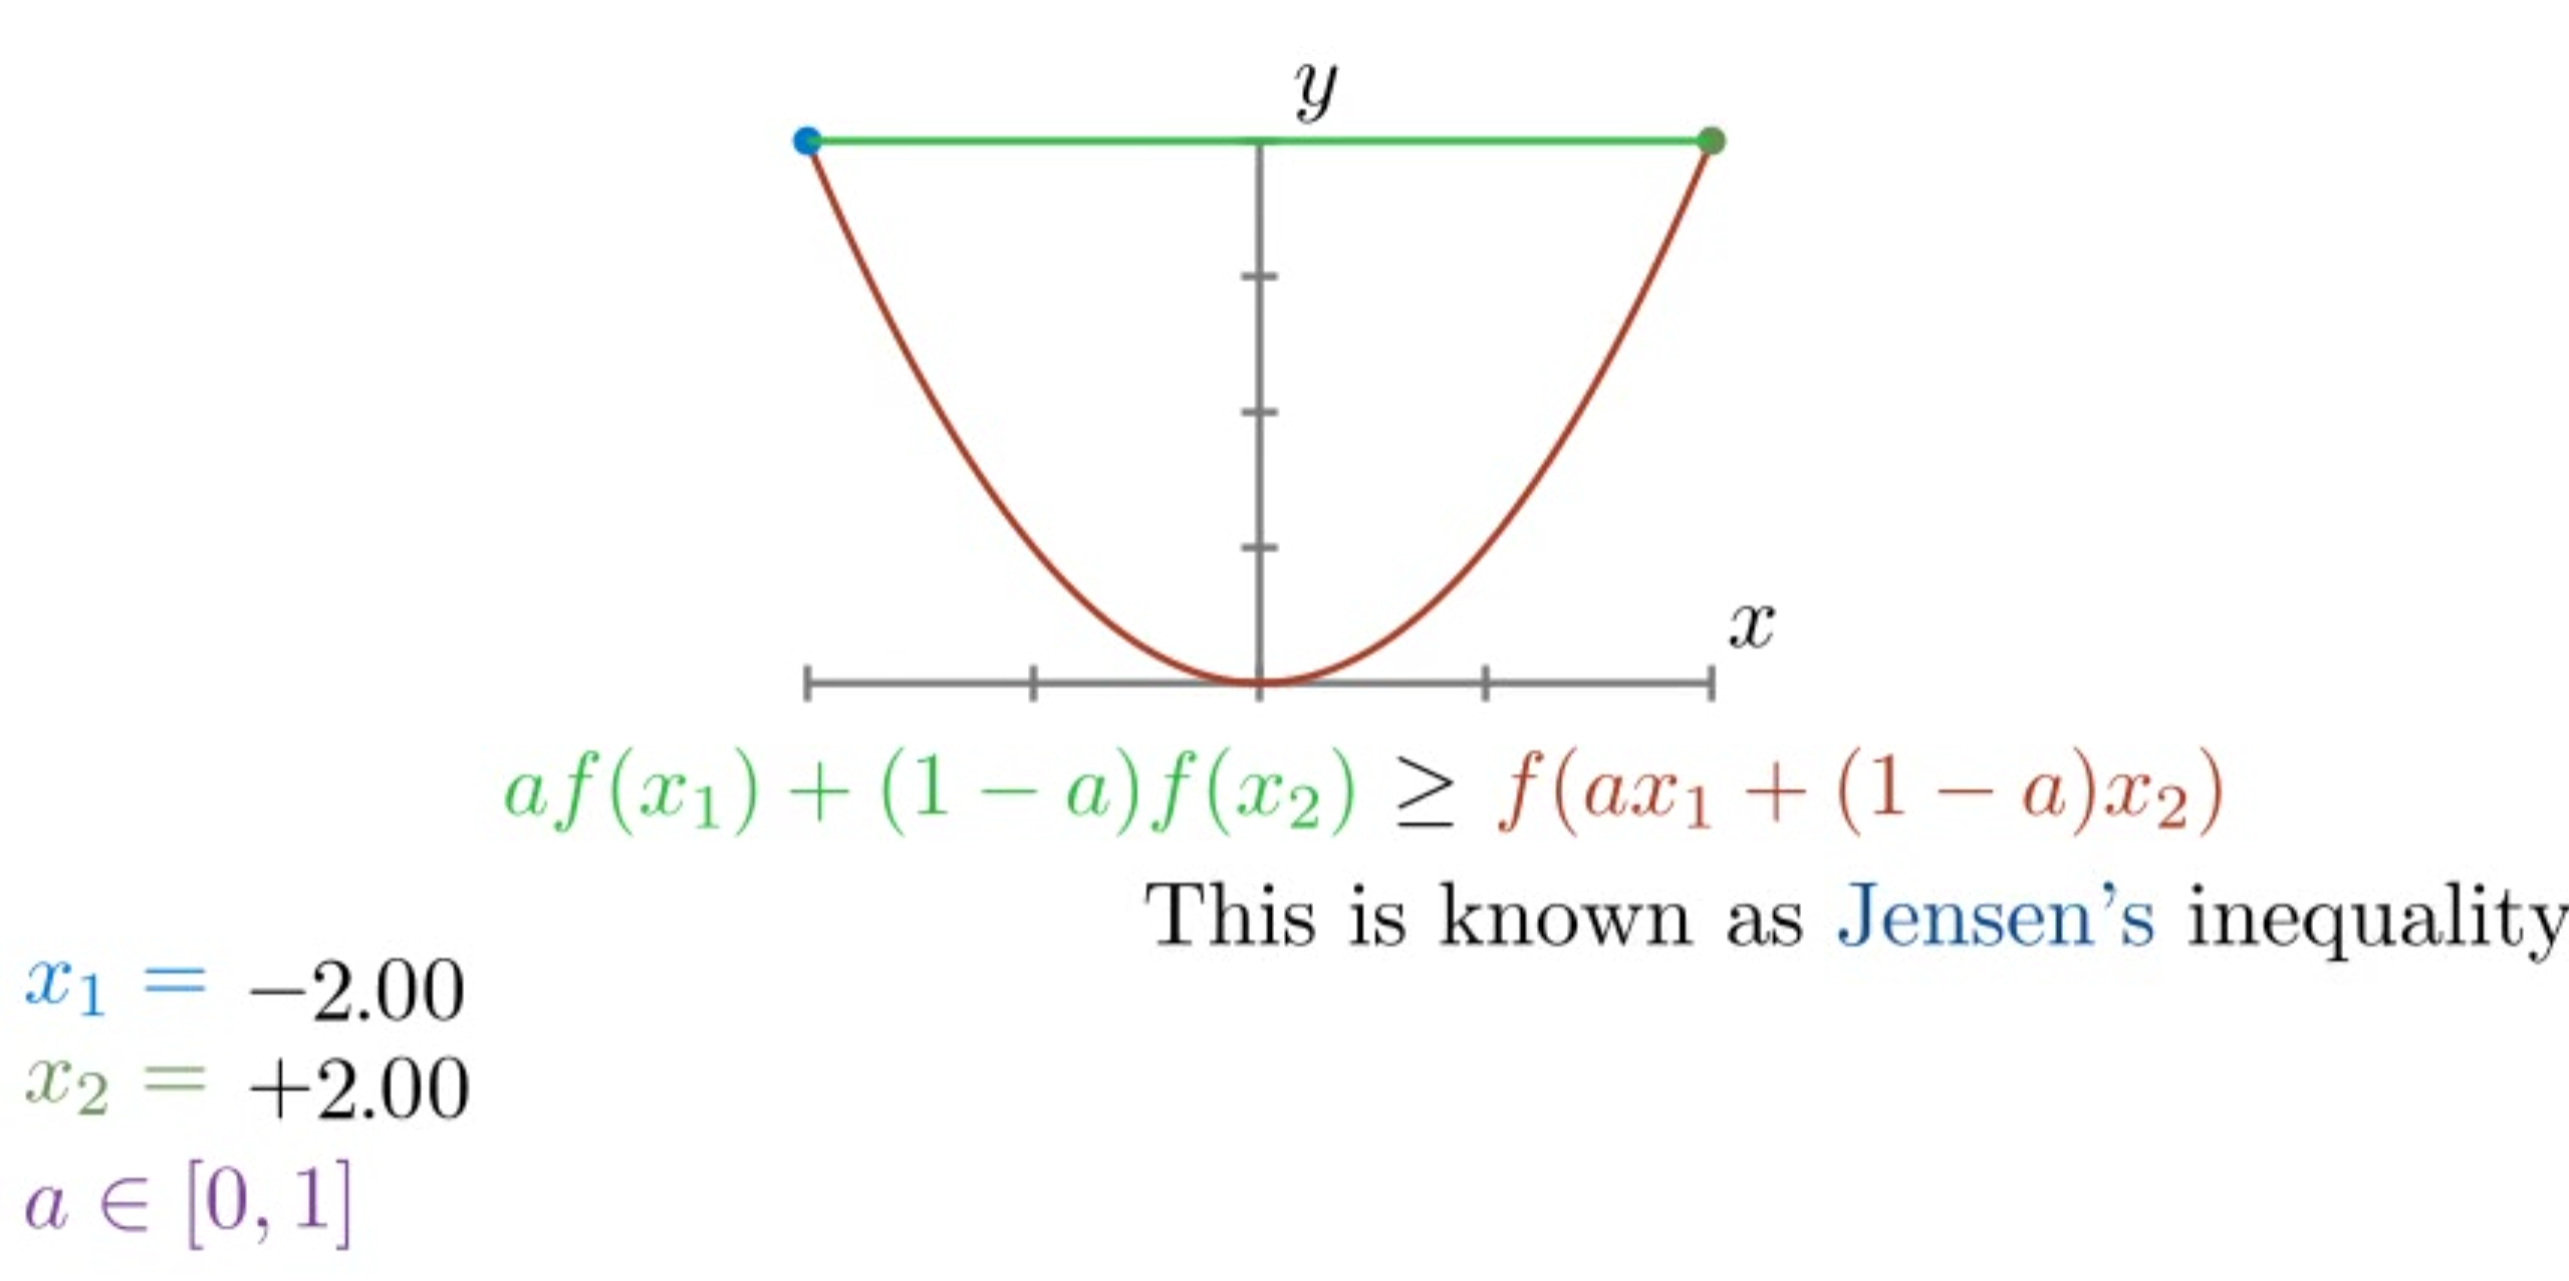
\includegraphics[scale=0.2]{images/convex1}
\end{itemize}
\end{itemize}
\item Sample Mean and Variance (iid)
\begin{itemize}
\item Sample Variance: $S^{2}=\frac{1}{n-1}{\displaystyle \stackrel[i=1]{n}{\sum}(x_{i}-\bar{x})^{2}}$
\item Assume $E[x_{i}]=\mu$ and $Var[x_{i}=\sigma^{2}]$
\begin{itemize}
\item $E(\bar{x})=\mu$, $Var(\bar{x})=\frac{\sigma^{2}}{n}$
\item $E(S^{2})=\sigma^{2}$
\end{itemize}
\end{itemize}
\item Sample Mean and Variance of Normal population (iid)
\begin{itemize}
\item $\bar{x}$ and $S^{2}$ are independent
\item $\bar{x}\sim N(\mu,\frac{\sigma^{2}}{n})$
\item $\frac{(n-1)S^{2}}{\sigma^{2}}\sim\chi_{n-1}^{2}$
\end{itemize}
\item Power function $\beta(\theta)=P_{\theta}(\boldsymbol{X}\in R)$, define
rejection region
\begin{itemize}
\item A test with power function $\beta(\theta)$ is \textbf{size} $\alpha$
test if $\underset{\boldsymbol{\theta\in\Theta_{0}}}{\text{sup}}\beta(\theta)=\alpha$
and is \textbf{level} $\alpha$ test if $\underset{\boldsymbol{\theta\in\Theta_{0}}}{\text{sup}}\beta(\theta)\leq\alpha$
\end{itemize}
\item P-Value: If the rejection region is of the form $R=\{\boldsymbol{x}:T(\boldsymbol{X})>c\}$
then the P-Value is
\[
p(x)=\underset{\boldsymbol{\theta\in\Theta_{0}}}{\text{sup}}P_{\theta}(T(\boldsymbol{X})\geq t(\boldsymbol{x}))
\]

\begin{itemize}
\item NOTE: $T(\boldsymbol{X})$ is a random variable and this is the upper
limit under the null hypothesis, so the statistic $t(\boldsymbol{x})$
is evaluated at the sup of the null parameter.
\item Example for standard normal with critical value $t(\boldsymbol{X})=k_{1-\alpha}$,
i.e. the upper $\alpha$ quantile critical point of standard normal,
then $p(x)=P(T(\boldsymbol{X})\geq k_{1-\alpha})=1-\Phi(k_{1-\alpha})$
\item $p(x)=\underset{\theta\in\Theta_{0}}{\text{sup}}P_{\theta}(T(X)\leq t(x))$
for rejection regions of the form $R=\{\boldsymbol{x}:T(\boldsymbol{X})<c\}$
\end{itemize}
\item UMVUE
\begin{itemize}
\item Fisher information: $I_{n}(\theta)=-E_{\theta}\left(\frac{d^{2}}{d\theta^{2}}\log(L(\theta|\boldsymbol{x}))\right)$,
Cramer-Rao lower bound is $\frac{[\tau^{\prime}(\theta)]^{2}}{I_{n}(\theta)}$
which for i.i.d sample is $\frac{[\tau^{\prime}(\theta)]^{2}}{nI(\theta)}$
\item Attainment: $a(\theta)[W(\boldsymbol{X})-\tau(\theta)]=\frac{d}{d\theta}\log(L(\theta\boldsymbol{|x})$,
where $W(\boldsymbol{X})$ is estimator for $\tau(\theta)$ ($E_{\theta}(W(\boldsymbol{X}))=\tau(\theta))$
look at $a(\theta)W(\boldsymbol{X})-a(\theta)\tau(\theta)$
\item Lehmann-Scheffe: $g(s(\boldsymbol{x}))=E[t(\boldsymbol{x})|s(\boldsymbol{x})]$,
where $g(s(\boldsymbol{x}))$ is UMVUE, $t(\boldsymbol{x})$ is an
unbiased (usually crude) statistic, and is conditioned with complete
sufficient statistic $s(\boldsymbol{x})$.
\end{itemize}
\item Aymptotic Properties of MLE: assume regularity conditions. Let $\theta^{*}$
be the true value of $\theta$. For an MLE $\hat{\theta}=\hat{\theta}_{n}$
of $\theta$, we have that
\begin{itemize}
\item (uniqueness) $\hat{\theta}_{n}$ is unique
\item (consistent) $\hat{\theta}_{n}\overset{p}{\rightarrow}\theta^{*}$
\item (asymptotically unbiased) $\underset{n\rightarrow\infty}{\lim}E(\hat{\theta}_{n})=\theta^{*}$
\item (asymptotically efficient) $Var(\hat{\theta}_{n})\rightarrow CRLB_{\theta}$
as $n\rightarrow\infty$
\item (asymptotically normal) $\hat{\theta}_{n}\overset{asym}{\sim}N(\theta^{*},CRLB_{\theta})$ 
\item Confidence Interval using $\hat{\theta}_{n}$

\[
P(-Z_{\frac{\alpha}{2}}\leq\frac{\hat{\theta}_{n}-\theta^{*}}{\sqrt{CRLB_{\theta}}}\leq Z_{\frac{\alpha}{2}})\approx1-\alpha
\]
\end{itemize}
\end{itemize}

\end{document}
